\begin{table}[ht]
\centering
\begin{tabular}{ccc}
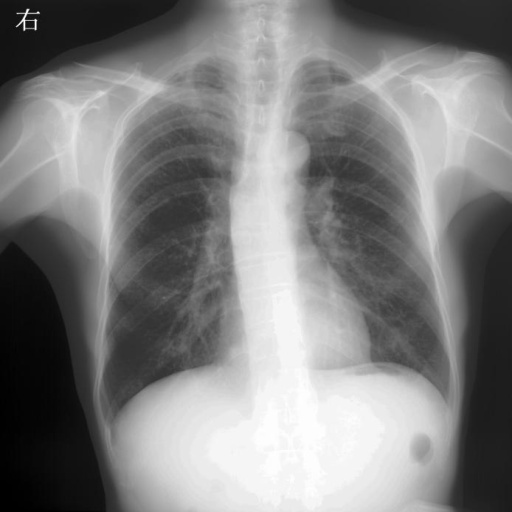
\includegraphics[width=0.2\textwidth]{main/content/images/dataset_comparison/pneumoconiosis/1.jpg} &
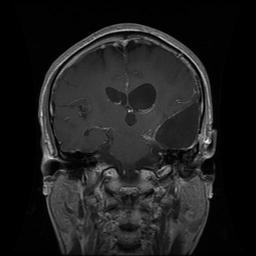
\includegraphics[width=0.2\textwidth]{main/content/images/dataset_comparison/brain_tumor/1.jpg} &
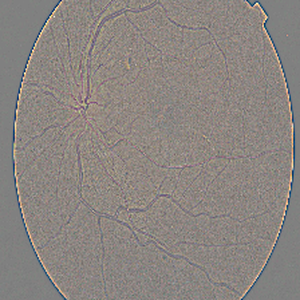
\includegraphics[width=0.2\textwidth]{main/content/images/dataset_comparison/retinopatia/1.png} \\
(a) X-ray - Image 1 & (b) MRI - Image 1 & (c) Scan - Image 1 \\
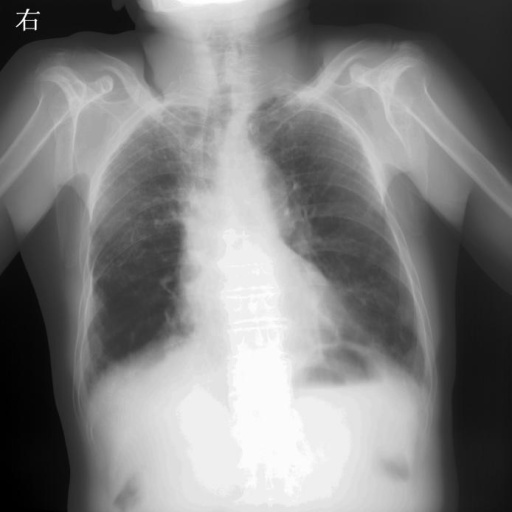
\includegraphics[width=0.2\textwidth]{main/content/images/dataset_comparison/pneumoconiosis/2.jpg} &
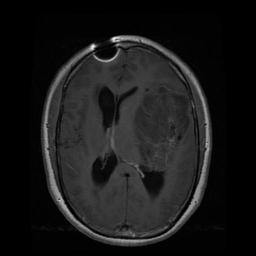
\includegraphics[width=0.2\textwidth]{main/content/images/dataset_comparison/brain_tumor/4.jpg} &
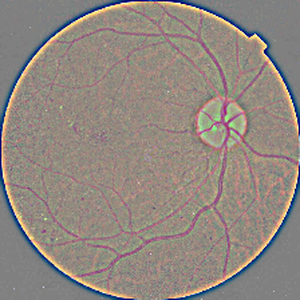
\includegraphics[width=0.2\textwidth]{main/content/images/dataset_comparison/retinopatia/2.png} \\
(d) X-ray - Image 2 & (e) MRI - Image 2 & (f) Scan - Image 2 \\
\end{tabular}
\caption{Image diversity among and within datasets.}
\label{tab:image_diversity}
\end{table}